\section{Постановка задачи. Необходимая теория}
\label{sec:theory}

% Расскажем об импульсных динамических системах подробнее и подведем %
% соотв. теоретическую базу.
%\section {Импульсные управления}
\subsection {Уравнение эйконала}
\label{sec:csdisttrack}

Предположим - у нас есть некоторая граница (замкнутая кривая в
двумерном пространстве), разделяющая область $\Omega$ на две подобласти:
внутреннюю и внешнюю. Предположим также, что кривая распространяется с
известной скоростью $F$, как показано на рисунке~\ref{fig:eikvis}. Для наших
потребностей достаточно предположить, что кривая расширяется, т.е. ее
движение направлено вовне текущей области $(F>0)$, а также
игнорируется касательная компонента движения, т.е. кривая
распространяется только по нормальному вектору, определенному $F$:

\begin{figure}[h]
  \centering
  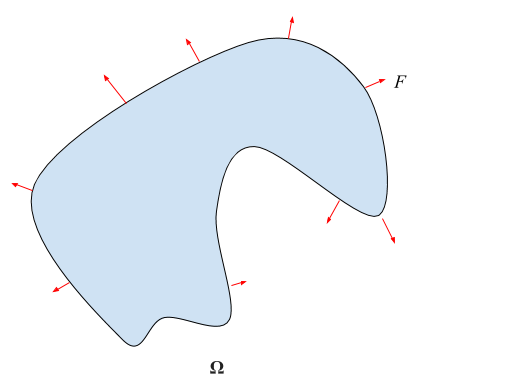
\includegraphics[width=0.5\linewidth]{img/eikonal_vision.png}
  \hfil \caption{распространение кривой со скоростью $F$}
  \label{fig:eikvis}

\end{figure}


Для того, чтобы определить положение кривой в каждой точке области. Мы
можем вычислить время прибытия $T$, когда впервые будет пересечена
каждая из точке $(x,y)$.

Если взять одномерный случай, то там мы можем вычислять расстояние как
произведение скорости на время, тогда мы можем записать уравнение для
функции $T$:

\begin{equation*}
  1 = F \frac{dT}{dx}
\end{equation*}

В пространствах более высокой размерности время прибытия T это решение
краевой задачи , также называемой уравнением эйконала.

\begin{equation}
  \label{eq:eikonal}
  \left\{ \begin{matrix}
      F(x) || \nabla T(x) || = 1, x \in \Omega \\
      T(x) = 0, x \in \Gamma
    \end{matrix}\right.
\end{equation}

Здесь $\Omega$ -- это область в $\mathbb{R}^n$, $\Gamma$ -- начальная
позиция кривой, $\nabla$ обозначает градиент, и $\|| \cdot ||$ является
Евклидовой нормой.

Стоит отметить, что эволюция кривой и время первого прибытия
отличаются. Для иллюстрации рассмотрим распространение кривой со
скоростью $F \equiv 1$, как представлено на Рисунке~\ref{fig:prpgt-eik}

\begin{figure}[h]
  \centering
  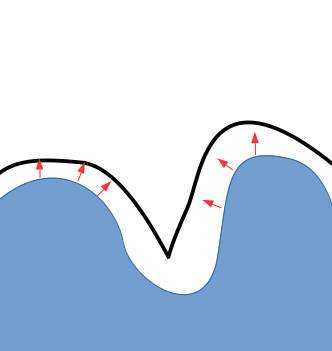
\includegraphics[width=0.3\linewidth]{img/propagate_eikonal.png}
  \hfil \caption{распространение кривой со скоростью $F = 1$}
  \label{fig:prpgt-eik}

\end{figure}

Жирная линия указывает где будет кривая на следующем шаге.  Предположим
теперь мы хотим заглянуть дальше, тогда мы получим следующую картину
на рисунке~\ref{fig:swallow-ex} кривая пройдет сквозь себя, соорудив
так называемый \textit{ласточкин хвост}. Чем он плох? Мы в некоторых
точках получаем многозначную функцию, чего нужно избегать. В
\cite{S1999}, Сетиан описывает эту ситуацию, как если мы рассмотрим
фронт распространения кривой, как фронт распространения огня, тогда
то, что было однажды сожжено, второй раз не сжигается.  Следовательно
нам стоит выбрать в каком-то смысле физически корректное решение с
фигурой, как на рисунке~\ref{fig:correct-exmp}

\begin{figure}[h]
  \centering
  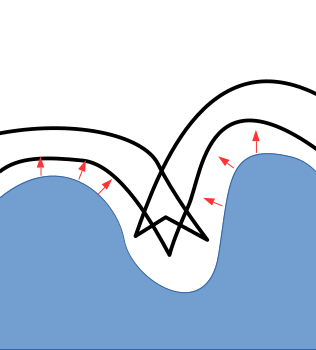
\includegraphics[width=0.3\linewidth]{img/swallow-tail-example.png}
  \hfil \caption{Пример ласточкиного хвоста}
  \label{fig:swallow-ex}

\end{figure}

\begin{figure}[h]
  \centering
  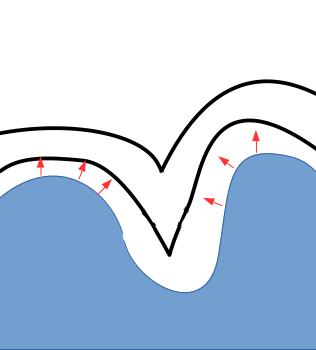
\includegraphics[width=0.3\linewidth]{img/corrct-example.png}
  \hfil \caption{Пример корректного решения}
  \label{fig:correct-exmp}

\end{figure}

Уравнение~\eqref{eq:eikonal} является частным случаем \textit{уравнения
Гамильтона-Якоби} первого порядка, которое в статичном случае выглядит
следующим образом:

\begin{equation}
  \label{eq:hje}
  \left\{ \begin{matrix}
      H(x, Du) = 0,\text{на } \mathbb{R}^n \times (0,\infty) \\
      T(x) = 0,  \text{на } \mathbb{R}^n \times \{t = 0\},
    \end{matrix}\right.
\end{equation}
где Гамильтониан $H = H(x,Du)$ непрерывная вещественная функция на
$\mathbb{R}^n \times \mathbb{R}^n$ и $\phi : \mathbb{R}^n \rightarrow
\mathbb{R}$ -- начальная функция.

В общем случае это уравнение не имеет классических $C^1$
решений. Проблема эта имеет решение в обобщенных решениях, которые
непрерывны и удовлетворяют данному уравнению в частных производных
почти всюду.

%%% Local Variables:
%%% mode: latex
%%% TeX-master: "eikonal_solver"
%%% End:
